%!TEX root = ../DSGEnotes.tex
\section{数值求积}
\label{sec:numerical-integration-ncrule}

我们常常需要计算一个定积分的值,如
\begin{equation*}
  \int_{a}^{b} f(x) \, \mathrm{d}x,
\end{equation*}
若直接用解析法求解较为困难,则常常采取数值积分(numerical integratation)\index{numerical integration \dotfill 数值积分}的思路,将积分式转化为有限个方程求和的方式做近似求解,如
\begin{equation}
  \label{eq:nint-num-integ-def}
  \int_{a}^{b} f(x) \, \mathrm{d} x \approx \sum_{n=1}^{N} w_{n} f \left( x_{n} \right),
\end{equation}
也即,我们在原方程的取值区间$[a,b]$中抽取$N$个点,$n=0,1,\ldots,N$的$x_{n}$值代回方程中对应值$f \left(x_{n} \right)$。$w_{n}$表示相应的权重系数。

因此,数值积分也常常称为数值求积(numerical quadrature)\index{numerical quadrature \dotfill 数值求积}。集合$\left\{ x_{n} \right\},\left\{ w_{n} \right\}$常常称为求积点(quadrature points)\index{quadrature points \dotfill 求积点}集合和求积权重(quadrature weights)\index{quadrature weights \dotfill 求积权重}集合;合适的选取$\left\{ x_{n} \right\},\left\{ w_{n} \right\}$的算法称为求积法则(quadrature rule)\index{quadrature rule \dotfill 求积法则}。对于同一个积分求解问题\eqref{eq:nint-num-integ-def}往往存在一系列法则;评价不同法则之间好坏的标准在于,看哪个法则能用最少的样本点$N$来对\eqref{eq:nint-num-integ-def}作出最精确的近似,同时确保计算成本可控,如编程难度、计算时间等。

先从最基本的牛顿——寇特斯法则开始介绍。

\subsection{牛顿——寇特斯法则}
\label{sec:nint-nc-rule}
近似求解积分问题\eqref{eq:nint-num-integ-def}的基本思路是,在区间$[a,b]$中找到一个多项式方程$P(x)$来近似$f(x)$。由于多项式的求和计算往往较为简单(多项式的介绍见第\ref{sec:poly}节),这会简化\eqref{eq:nint-num-integ-def}RHS的计算时间。我们将这种思路称为牛顿——寇特斯(求积)法则(Newton—Cotes Rule)\index{Newton—Cotes Rule \dotfill 牛顿——寇特斯法则}。牛顿——寇特斯法则随着多项式的次(degree, order)而呈层级特征:使用$p$次多项式的牛顿——寇特斯法则可称为$p$阶牛顿——寇特斯法则。

如果$f$不是多项式,那么在$[a,b]$区间内寻找近似多项式$P(x)$会较为困难。一个近似方案是将空间$[a,b]$划分为$N$个子区间(对应$N+1$个点),在每个子空间中分别寻找可以近似$f$的多项式,进而将多个多项式加权求和,作为整个空间中$f$的近似方程。$N$越大,子空间的个数越多,划分就越精细,每个子空间中的近似就越精确,进而整个空间中的近似求积就越精确。

\subsubsection{矩形法则}
\label{sec:ninc-nc-rectangular-rule}
我们先从$p=0$的情况开始理解牛顿——寇特斯法则,根据黎曼求和(Riemann sums),我们可以将方程$f(x)$理解为一组矩形的集合,对$f(x)$在区间$[a,b]$中求积就是求曲线下方的面积,近似等于各个矩形面积的和。随着$N$趋近于无穷大,每个矩形的宽度无限接近于$0$,近似就越精确。

在每个子空间中分别用$1$个$p=0$次多项式来近似$f$,$0$次多项式是个常数,换句话说我们在每个子空间中用一个常数来近似$f$。这又称为矩形求积法则(rectangular quadrature rule)\index{rectangular (quadrature) rule \dotfill 矩形(求积)法则}。

\begin{figure}[htbp]
   \caption{矩形法则$(N=4)$}
  \centering
  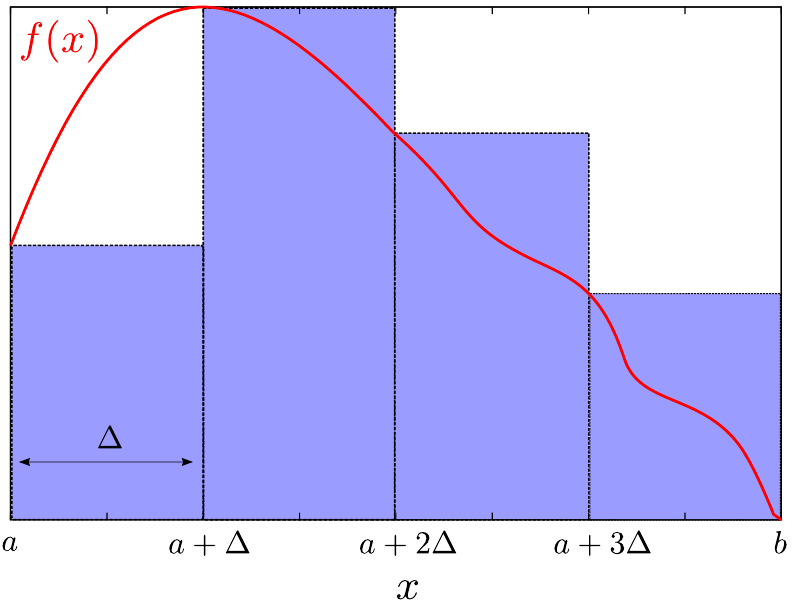
\includegraphics[width=8cm]{./Figures/20180227-rectangular-rule-example.png}
  \label{fig:ninc-nc-rectangular-rule}
%
%  \small{Source: PBOC.}
\end{figure}
图\ref{fig:ninc-nc-rectangular-rule}绘出了$N=4$情况下,利用矩形法则对$\int_{a}^{b} f(x) \, \mathrm{d}x$的近似。不难看出,将区间$[a,b]$划分为$N$个等宽子区间,每个子区间的宽度都是$\Delta = \left(b - a \right)/N$。最左侧第一个矩形,左边长(高)为$f(a)$,宽为$\Delta$,对应面积为$f(a) \cdot \Delta$。
左数第二个矩形,左边长(高)为$f \left( a+\Delta \right)$,宽也是$\Delta$,面积为$\left( a+\Delta \right) \cdot \Delta$,以此类推直到第$N=4$个矩形为止。将这些子区间中矩形的面积加总,可得矩形法则的近似表达式
\begin{equation*}
    \mathcal{I}_{N=4}^{rect}
    %\mathcal{N}_{N=4}^{rect}
    \approx
    f(a) \cdot \Delta
    + f \left(a + \Delta \right) \cdot \Delta
    + f \left(a + 2 \Delta \right) \cdot \Delta
    + f \left(a + 3 \Delta \right) \cdot \Delta,
\end{equation*}
扩展到更一般的$N \in \mathcal{N}$的情况,利用$N$段矩形法则对积分$\int_{a}^{b} f(x) \, \mathrm{d} x$的近似为
\begin{equation}
  \label{eq:ninc-nc-rectangular-rule}
  \mathcal{I}_{N}^{rect} = \sum_{n=0}^{N-1} f \left( a + n \cdot \Delta \right) \cdot \Delta.
\end{equation}

矩形法则\eqref{eq:ninc-nc-rectangular-rule}成为对\eqref{eq:nint-num-integ-def}的近似求积法则之一:
\begin{itemize}
  \item 求积权重集合$\left\{ w_{n} \right\}_{n=0}^{N-1}$对应$w_{n} \equiv \Delta \, \forall \, n$,
  \item 求积点集合$\left\{ x_{n} \right\}_{n=0}^{N-1}$对应$x_{n} = a + n \cdot \Delta, \, n = 0,1,\ldots,N-1$。
\end{itemize}

值得注意的是,在矩形法则下,我们只需要左边长,从而无需计算$f(b)$。


\subsubsection{梯形法则}
\label{sec:ninc-nc-trapezoidal-rule}
从图\ref{fig:ninc-nc-rectangular-rule}中不难看出,利用矩形法则近似曲线下方阴影的面积,近似效果并不理想。一个可能的改进方案是利用梯形代替矩形做近似,又称梯形近似法则。

在每个子空间中分别用$1$个$p=1$次多项式来近似$f$,$1$次多项式是条斜线,连接子区间的两个端点(始点和终点)。这又称为梯形求积法则(trapezoidal quadrature rule)\index{trapezoidal (quadrature) rule \dotfill 梯形(求积)法则}。

\begin{figure}[htbp]
  \caption{梯形法则$(N=4)$}
  \centering
  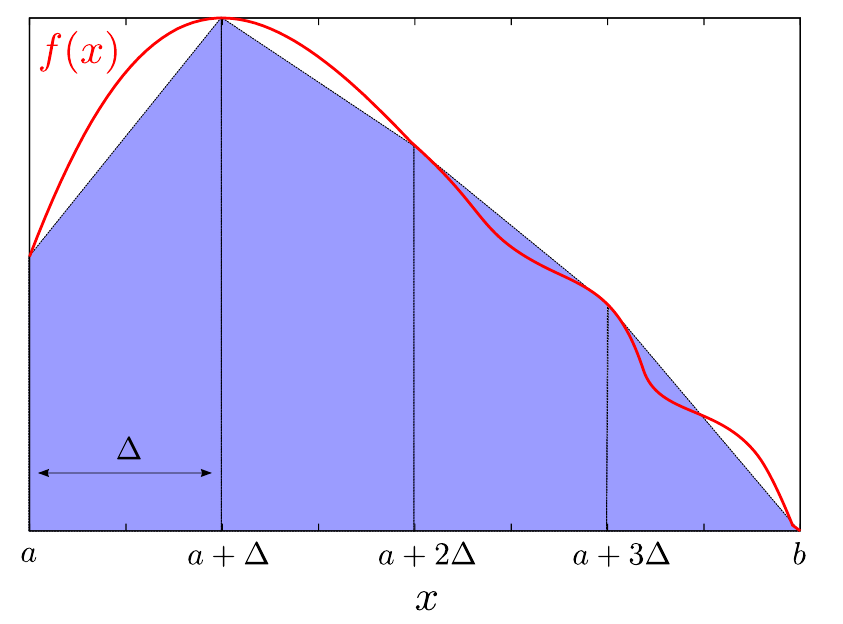
\includegraphics[width=8cm]{./Figures/20180227-trapezoidal-rule-example.png}
  \label{fig:ninc-nc-trapezoidal-rule}
%
%  \small{Source: PBOC.}
\end{figure}

见图\ref{fig:ninc-nc-trapezoidal-rule}所示,左数第$1$个梯形的面积等于
\begin{equation*}
  \frac{1}{2} \left[ f \left( a \right) + f \left( a + \Delta \right) \right] \cdot \Delta,
\end{equation*}

左数第$2$个梯形的面积等于
\begin{equation*}
  \frac{1}{2} \left[ f \left( a + \Delta \right) + f \left( a + 2 \Delta \right) \right] \cdot \Delta,
\end{equation*}
以此类推直到第$N=4$个梯形。将子区间中梯形的面积加总,可得
\begin{equation*}
\begin{split}
  \mathcal{I}_{N=4}^{trap} = &
    \frac{1}{2} \left[ f \left( a \right) + f \left( a + \Delta \right) \right] \cdot \Delta
    + \frac{1}{2} \left[ f \left( a + \Delta \right) + f \left( a + 2 \Delta \right) \right] \cdot \Delta \\
    & + \frac{1}{2} \left[ f \left( a + 2 \Delta \right) + f \left( a + 3 \Delta \right) \right] \cdot \Delta
    + \frac{1}{2} \left[ f \left( a + 3 \Delta \right) + f \left( a + 4 \Delta \right) \right] \cdot \Delta \\
    = & \left[
    \frac{1}{2} f \left( a \right)
    + f \left( a + \Delta \right)
    + f \left( a + 2 \Delta \right)
    + f \left( a + 3 \Delta \right)
    + \frac{1}{2} f \left( a + b \right)
    \right] \cdot \Delta,
\end{split}
\end{equation*}
扩展到更一般的$N \in \mathcal{N}$的情况,我们有$N$段梯形法则对$\int_{a}^{b} f \left( x \right) \, \mathrm{d} x$的近似为
\begin{equation}
  \label{eq:ninc-nc-trapezoidal-rule}
  \mathcal{I}_{N}^{trap} = \frac{1}{2} f \left( a \right) \cdot \Delta
  + \Delta \cdot \sum_{n=1}^{N-1} f \left( a + n \cdot \Delta \right)
  + \frac{1}{2} f \left( b \right) \cdot \Delta.
\end{equation}


梯形法则\eqref{eq:ninc-nc-trapezoidal-rule}称为对\eqref{eq:nint-num-integ-def}的又一种近似求积法则:
\begin{itemize}
  \item 求积点集合$\left\{ x_{n} \right\}_{n=1}^{N-1}$对应$x_{n} = a + n \cdot \Delta, \, n = 0,1,\ldots,N$,
  \item 求积权重集合$\left\{ w_{n} \right\}_{n=1}^{N}$对应
  \begin{equation*}
  w_{n} =
  \begin{cases}
  \frac{1}{2} \Delta, & n = 0, N, \\
  \Delta, & n = 1, 2, \ldots, N-1,
  \end{cases}
\end{equation*}
值得注意的是,比起矩形法则来,当利用梯形法则做近似求积时,需计算$N+1$个求积抽样点,比矩形法则多出的$1$个点为总区间中的末端$b$,对应$f(b)$。
\end{itemize}

\subsubsection{更高阶牛顿——寇特斯法则}
\label{sec:ninc-nc-higher-rule}
已知用$p=0$阶多项式(常数)近似子区间中的$f$,称矩形法则。用$p=1$阶多项式(斜线)近似,称梯形法则。那么我们可以进一步迭代计算更高阶$p > 1$的牛顿——寇特斯求积近似,方法如下
\begin{enumerate}
  \item 在子区间$\left[ x_{n}, x_{n+1} \right]$中,配$p+1$个等距离分布的点(包括子区间的起始点$x_{n}$和终结点$x_{n+1}$),将子区间分为$p$个部分。例如,
  \begin{itemize}
    \item 对$p=2$而言,配3个点$x_{n}, \frac{1}{2} \cdot \left[ x_{n} + x_{n+1} \right] , x_{n+1}$,
    \item 对$p=3$而言,配4个点$x_{n}, \frac{1}{3} \cdot \left[ x_{n} + x_{n+1} \right] , \frac{2}{3} \cdot \left[ x_{n} + x_{n+1} \right], x_{n+1}$,以此类推。
  \end{itemize}
  \item 在子空间中针对这$p+1$个配点,找到唯一的多项式$P(x)$以近似$f(x)$。例如,
  \begin{itemize}
    \item $p=0$,$P(x)$是个常数。矩形法则。
    \item $p=1$,$P(x)$是条斜线,连接子区间的两个端点$f \left( x_{n} \right), \, f \left( x_{n+1} \right)$。梯形法则。
    \item $p=2$,$P(x)$是一条经过如下3个点的抛物线,3个点的坐标依次为
    \begin{equation*}
      \begin{cases}
        \Big( x_{n}, f \left( x_{n} \right) \Big), \\
        \Big( x_{m}, f \left( x_{m} \right) \Big), \quad x_{m} \equiv \frac{x_{n} + x_{n+1}}{2}, \\
        \Big( x_{n+1}, f \left( x_{n+1} \right) \Big).
      \end{cases}
    \end{equation*}
    \item $p=3$,$P(x)$是一条经过如下4个点的曲线(图\ref{fig:ninc-nc-higher-p3}),4个点的坐标依次为
    \begin{equation*}
      \begin{cases}
        \Big( x_{n}, f \left( x_{n} \right) \Big), \\
        \Big( x_{m}, f \left( x_{m} \right) \Big), \quad x_{m} \equiv \frac{1}{3} \left( x_{n} + x_{n+1} \right), \\
        \Big( x_{m+1}, f \left( x_{m+1} \right) \Big), \quad x_{m+1} \equiv \frac{2}{3} \left( x_{n} + x_{n+1} \right), \\
        \Big( x_{n+1}, f \left( x_{n+1} \right) \Big),
      \end{cases}
    \end{equation*}
    \begin{figure}[htbp]
       \caption{3阶牛顿——寇特斯法则,对应子区间中的4个配点}
      \centering
      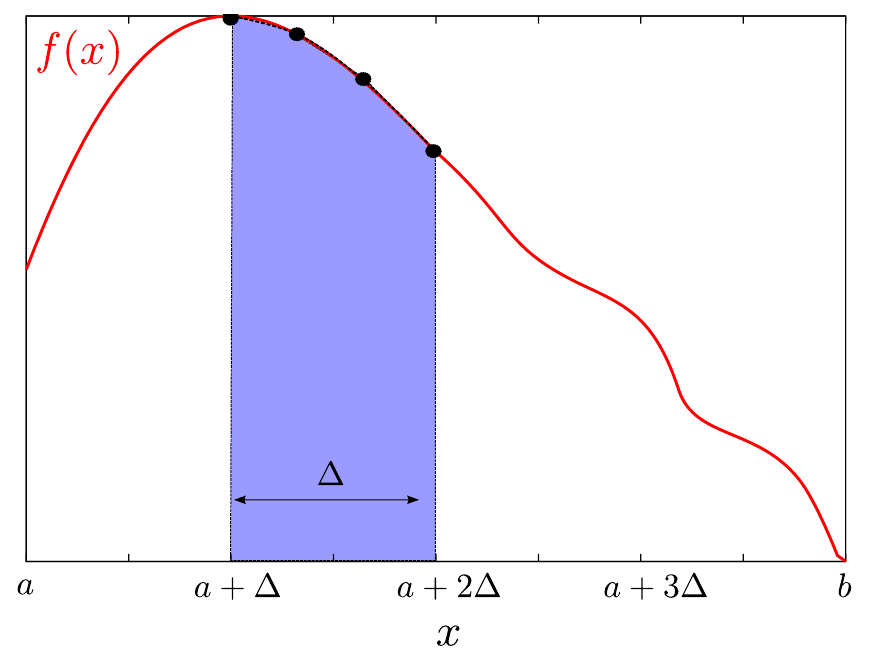
\includegraphics[width=8cm]{./Figures/20180227-nc-higher.png}
      \label{fig:ninc-nc-higher-p3}
    %
    %  \small{Source: PBOC.}
    \end{figure}
以此类推。无论哪一个例子中,$P(x)$都是这样一个多项式,其系数是抽样方程$f(x)$值的线性组合。
  \end{itemize}

  \item 从$x_{n}$到$x_{n+1}$对$P(x)$求积分,作为这个子区间内方程$f(x)$的近似。
  \item 将所有子区间内的近似方程组合起来,作为总区间中的最终近似求积法则。
\end{enumerate}

$p=2$时的牛顿——寇特斯求积,又称辛普森法则(Simpson's rule)\index{Simpson's (quadrature) rule \dotfill 辛普森(求积)法则}
\begin{equation}
  \label{eq:ninc-nc-simpson-rule}
  \mathcal{I}_{N}^{simp} =
  \sum_{n=0}^{N-1}
  \frac{\Delta}{6}
  \left[
  f \left( a + n \cdot \Delta \right)
  + 4 f \left( a + \left( n + \frac{1}{2} \right) \cdot \Delta \right)
  + f \left( a + \left( n + 1 \right)  \right) \cdot \Delta
  \right].
\end{equation}

\subsubsection{龙格现象}
\label{sec:ninc-nc-runge}
%20180227-Runge-phenomenon.png
一个自然出现的问题:更高阶的牛顿——寇特斯法则会不会带来更精确的近似解?很遗憾,答案是否定的。这是由于龙格现象(Runge phenomenon)\index{Runge phenomenon \dotfill 龙格现象}:当我们试图利用子空间中等距分布的点做更高阶多项式近似时,再查指点附近的多项式方程会出现较大幅度的震荡,从而影响最终求积估计的精确度,可参考\href{https://en.m.wikipedia.org/wiki/Runge%27s_phenomenon}{维基百科词条}。图\ref{fig:ninc-nc-higher-runge-phenomenon}中,蓝线和绿线分别表示$p=5$和$p=9$时的差值多项式近似,对应$N=6$。红线表示龙格方程(Runge function)。

\begin{figure}[htbp]
   \caption{龙格现象$(N=6)$}
  \centering
  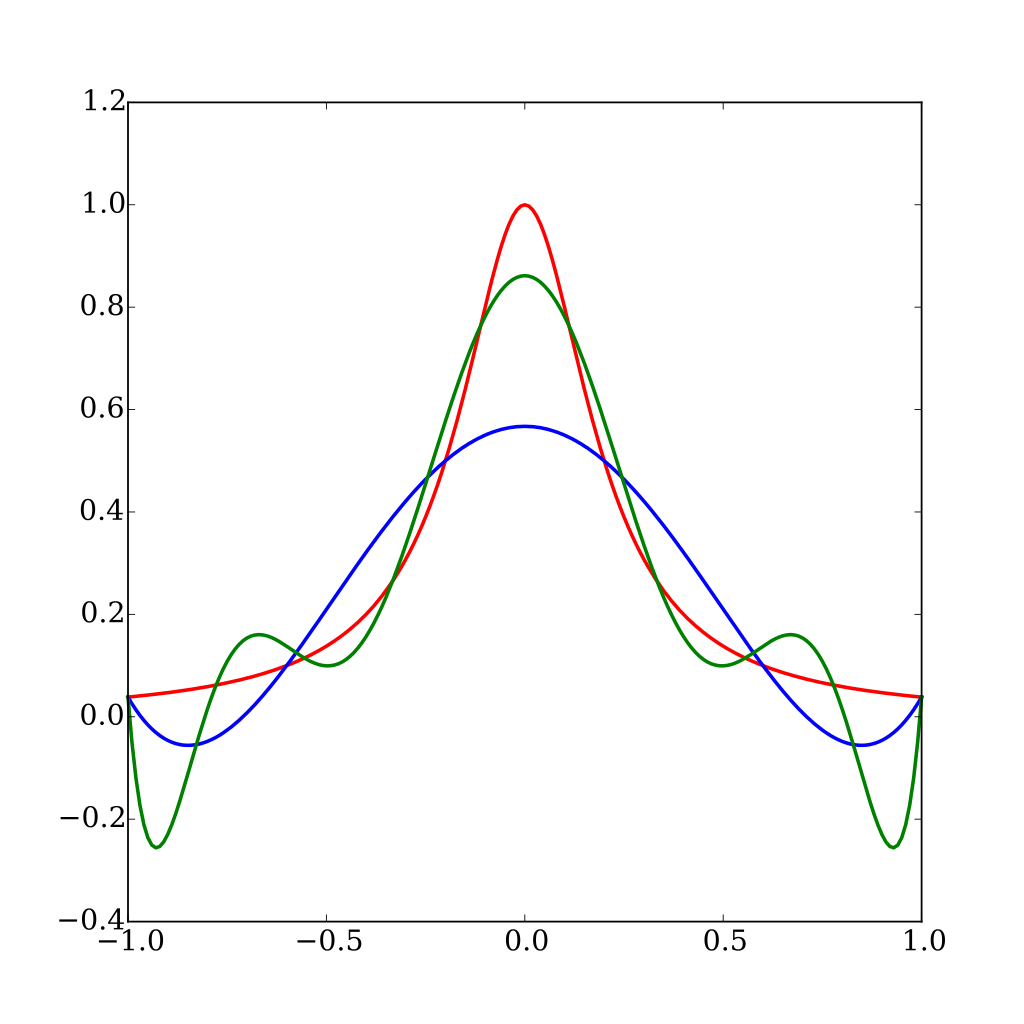
\includegraphics[width=8cm]{./Figures/20180227-Runge-phenomenon.png}
  \label{fig:ninc-nc-higher-runge-phenomenon}
%
%  \small{Source: PBOC.}
\end{figure}

\subsubsection{误差的收敛}
\label{sec:ninc-nc-error-convergence}
比较不同求积法则的优劣,可用启发式误差“分析”\footnote{加上引号是指,这种方法只是一种较为常用的检验措施,而不宜理解为某种严谨的学术性系统性表达。},观察近似误差随着配点数$N$增加的衰减速度。具体说来
\begin{enumerate}
  \item 考虑区间中某一宽度为$\Delta$的特定子区间,在其中用一个$p$阶多项式$P(x)$来近似$f$
  \begin{equation*}
    P(x) = c_{0} + c_{1} x + c_{2} x^{2} + \ldots + c_{p} x^{p}.
  \end{equation*}
  \item 那么子区间中存在一个点$x_{0}$,使得$f$围绕$x_{0}$做泰勒级数展开的前$p+1$项,与$P(x)$一致
  \footnote{例如
  \begin{itemize}
    \item $p=0$,矩形法则,$x_{0}$可以是子区间的起始点。
    \item $p=1$,梯形法则,$x_{0}$的存在性可由中值定理予以证明:$x_{n}$和$x_{n+1}$之间必然存在一点,该点上的方程值$f\left( x_{0} \right)$的导数,等于连接$f \left(x_{n} \right)$和$f \left( x_{n+1} \right)$两点的斜线的斜率。
    \item $p >1$,更高阶求和法则中$x_{0}$点存在性的证明,也可用类似思路证得。
  \end{itemize}
  }。
  可将$f$写成如下形式
  \begin{equation*}
    f(x) = \underbrace{
    c_{0} + c_{1} x + \ldots + c_{p} x^{p} }_{\equiv P(x)}
    + c_{p+1} x^{p+1} + \ldots.
  \end{equation*}
  \item 由此可见,原方程$f(x)$及其近似多项式$P(x)$之间的误差是一个从$p+1$阶开始的多项式
  \begin{equation*}
    f(x) - P(x) = c_{p+1} x^{p+1} + c_{p+2} x^{p+2} + \ldots,
  \end{equation*}
  \item 那么在这个子区间$\left[ x_{n}, x_{n+1} \right]$内的全部误差可求积得出
  \begin{equation*}
    \begin{split}
      \int \left[ f(x) - P(x) \right] \, \mathrm{d} x
      & = \int \left[
      c_{p+1} x^{p+1} + c_{p+2} x^{p+2} + \ldots \right] \, \mathrm{d} x \\
      & \propto \Delta^{p+2} + \text{更高阶项},
    \end{split}
  \end{equation*}
  最后一行是说,对$x^{p+1}$沿着某个宽度为$\Delta$的子区间求积,等于某个和$\Delta^{p+2}$成比例的值。
  \item 将一个子区间中的情况扩展到其他子区间,每个子区间中的误差项都与$\Delta^{p+2}$成定比例。更进一步地,由于$\Delta$与$N$反比例相关(N是整个区间中划分的子区间的数量)
  \begin{equation*}
    \Delta \sim \frac{1}{N},
  \end{equation*}
  那么每个子区间中的误差项可近似表示为
  \begin{equation*}
    \Delta \propto \frac{1}{N^{p+2}}.
  \end{equation*}
  \item 将$N$个子区间的误差项汇总
  \begin{equation}
    \varepsilon \propto \frac{N}{N^{p+2}} =  \frac{1}{N^{p+2}},
  \end{equation}
  例如矩形法则$(p=0)$的近似误差$\propto \frac{1}{N}$,梯形法则$(p=1)$的近似误差$\propto \frac{1}{N^{2}}$。可见误差与$N$成反比:$N$越大,划分的子区间数量越多,近似误差越小。
\end{enumerate}

举例,假定我们要用求积法则近似计算
\begin{equation*}
  \mathcal{I} = \int_{1}^{2} \log^{2} x \, \mathrm{d} x,
\end{equation*}
对应相对误差定义为$\varepsilon^{rel}$
\begin{equation*}
  \varepsilon^{rel} \equiv \frac{
  \big| \mathcal{I}_{N}^{approx} - \mathcal{I} \big|
  }{
  \mathcal{I}
  }
\end{equation*}

应用矩形法则和梯形法则,查看近似误差随着$N$增大的收敛情况如图\ref{fig:ninc-nc-error-convergence},可以看出

\begin{figure}[htbp]
   \caption{比较矩形法则和梯形法则下,近似误差随$N$值增大的收敛情况}
  \centering
  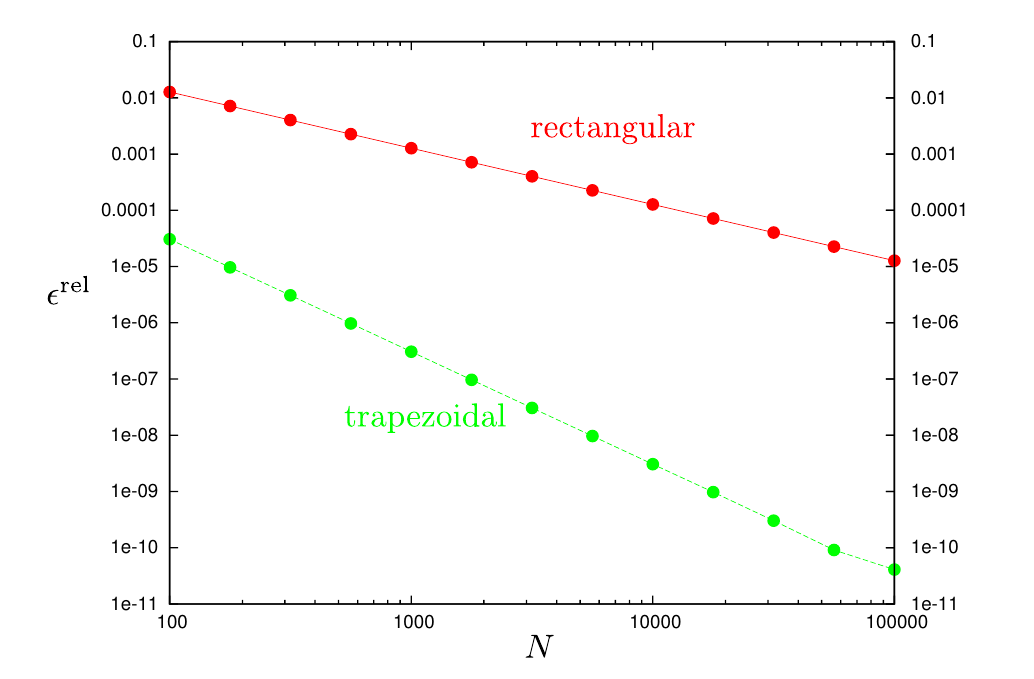
\includegraphics[width=10cm]{./Figures/20180227-nc-higher-error-convergence.png}
  \label{fig:ninc-nc-error-convergence}

  \small{原求积方程$\int_{1}^{2} \log^{2} x \, \mathrm{d} x$。}
\end{figure}

这两种方法代表的牛顿——寇特斯法则下误差项随着$N$而作线性收敛:
随着$N$增大$1,000$倍,矩形法则误差降低约$1,000$倍,$\Delta \varepsilon^{rect} \propto \frac{1}{\Delta N}$;梯形法则降低约$1,000,000$倍,$\Delta \varepsilon^{trap} \propto \frac{1}{ \left(\Delta N \right)^{2}}$。梯度法则优于矩形法则。

但图\ref{fig:ninc-nc-error-convergence}也揭示出牛顿——寇特斯法则的不足:即便是对于$\log^{2} x$这种很平滑的方程,梯形法则也需要大约$1,000$个样本,才能将总体误差控制在$10^{-6}$的水平上(为了达到类似的精度,矩形法则甚至需要$10^{6}$个样本)。从计算成本来看,牛顿——寇特斯法则恐怕不是最理想的方案,需要加以改进。如下文介绍的克伦肖——柯蒂斯法则,可以用少得多的样本量达到同样$10^{-6}$级别的误差水平,哪怕所处理的原方程更加复杂\todo{做一个ref}。

\subsection{几个小技巧}
\label{sec:ninc-tips}
以牛顿——寇特斯法则为例,介绍几个小技巧。它们对其他如克伦肖——柯蒂斯法则也适用。

\subsubsection{无限区间求积}
\label{sec:ninc-tips-improper-integral}
有时会遇到求含有无限区间的积分问题如
\begin{equation*}
  \int_{0}^{\infty} f(x) \, \mathrm{d} x,
\end{equation*}
这需要我们先将区间$[0, \infty)$映射到一个有界区间内,如
\begin{equation*}
  x:[0, \infty) \mapsto u:[0,1],
\end{equation*}
然后再应用求解定积分的求积法则。映射的方法有很多种,其中之一是设
\begin{equation*}
  x \equiv \frac{u}{1-u}, \Rightarrow \mathrm{d} x = \frac{\mathrm{d} u}{\left( 1 - u \right)^{2}},
\end{equation*}
求积问题因此转换为
\begin{equation*}
  \int_{0}^{\infty} f(x) \, \mathrm{d} x = \int_{0}^{1} \frac{1}{\left( 1 - u \right)^{2}} f
  \left( \frac{u}{1 - u} \right) \, \mathrm{d} u.
\end{equation*}

需要指出的是,上式在转换之后,含有一个奇异点(singularity):$\lim_{u \rightarrow 1} f(x) \rightarrow \infty$。然而若是在前提假设中假定$f(x)$在$x \rightarrow \infty$处消失(这个假定是为了确保积分$\int_{0}^{\infty} f(x) \, \mathrm{d} x$收敛),则这一奇异点也就不存在了。

\subsection{求积中的可积奇异点问题}
\label{sec:ninc-nc-singularity}
除了上节提到的情况之外,还应该注意到,有些奇异点是可积的(integrable singular points)\index{integrable singular points \dotfill 可积奇异点},例如这个求积问题
\begin{equation}
  \label{eq:ninc-nc-singularity-example}
  \mathcal{I} = \int_{0}^{1} \frac{\exp(x)}{\sqrt{x}} \, \mathrm{d} x,
\end{equation}
方程在区间$(0,1]$内定义良好,除了起始点$0$的情况,称之为可积奇异点\footnote{注意区分可积和不可积奇异点。后者如积分方程$\int_{0}^{1} \frac{\exp (x)}{x} \, \mathrm{d} x $的起始点$0$的情况,此时积分不存在,因此无法估计。}。存在可积奇异点的积分方程并不是全都不能求解,针对具体问题的不同,有一些求解技巧可供选择。试举例如下。

\subsubsection{提取奇异点}
\label{sec:ninc-nc-singularity-isolation}
有时可以在积分中把奇异点单独提取出来做求积运算,如  \eqref{eq:ninc-nc-singularity-example}可以改写为
\begin{equation*}
  \begin{split}
    \mathcal{I} & =
    \underbrace{
    \int_{0}^{1} \frac{1}{\sqrt{x}} \, \mathrm{d} x
    }_{\eqqcolon \mathcal{I}_{1}}
    + \underbrace{
    \int_{0}^{1} \frac{
    \exp (x) -1
    }{\sqrt{x}} \, \mathrm{d} x
    }_{\eqqcolon \mathcal{I}_{2}}.
  \end{split}
\end{equation*}

其中$\mathcal{I}_{1}$可以用解析法求得
\begin{equation*}
  \mathcal{I}_{1} = \int_{0}^{1} \frac{1}{\sqrt{x}} \, \mathrm{d} x = \big| 2 \sqrt{x} \big|_{0}^{1} = 2.
\end{equation*}

含有可积奇异点的$\mathcal{I}_{2}$无法用解析法求解,但在区间起始点($=0$)处是非奇异的:这是由于,将被积方程沿着$x \rightarrow 0$做泰勒级数展开,可得
\begin{equation*}
  \begin{split}
    & \frac{
    \exp (x) -1
    }{\sqrt{x}}
    \approx \frac{
    x - \frac{1}{2}x^{2} + \frac{1}{6} x^{3} + \ldots
    }{
    \sqrt{x}
    } = x^{\frac{1}{2}} - \frac{1}{2}x^{\frac{3}{2}} + \frac{1}{6} x^{\frac{5}{2}} + \ldots, \\
    & \hookrightarrow \lim_{x \rightarrow 0}
    \frac{
    \exp (x) -1
    }{\sqrt{x}} \rightarrow 0,
  \end{split}
\end{equation*}
因此可用常规求积法则进一步近似求解$\mathcal{I}_{2}$。

\subsubsection{奇异点消除}
\label{sec:ninc-nc-singularity-cancellation}
若被积方程的分母中含有可积奇异点,那么
可以考虑用雅各比变换(Jacobian transformation)
%\index{Jacobian transformation \dotfill 雅各比变换}
。例如对\eqref{eq:ninc-nc-singularity-example},设
\begin{equation*}
  u \equiv \sqrt{x} \Rightarrow \mathrm{d} u = \frac{\mathrm{d} x}{2 \sqrt{x}},
\end{equation*}
求积运算因此变为
\begin{equation*}
  \int_{0}^{1} \frac{\exp(x)}{\sqrt{x}} \, \mathrm{d} x= 2 \int_{0}^{1} \exp \left( u ^{2} \right) \, \mathrm{d} u,
\end{equation*}
新的积分方程中没有奇异点,因此可进一步用常规数值求积法则来近似。

\subsubsection{Epsilon扩展}
\label{sec:ninc-nc-singularity-epsilon-extension}
如果可积奇异点无法利用前述两种方法消除,我们可以尝试加入一个平滑参数$\epsilon$。对应地,取极限$\lim \epsilon \rightarrow 0$以消除奇异点。如将\eqref{eq:ninc-nc-singularity-example}改写为
\begin{equation*}
  \mathcal{I}_{\epsilon} = \int_{0}^{1}
  \frac{
  \exp (x)
  }{
  \left( x^{2} + \epsilon^{2} \right)^{\frac{1}{4}}
  } \, \mathrm{d} x.
\end{equation*}

对于有限值的$\epsilon < \infty$,上式非奇异,并且$\lim_{\epsilon \rightarrow 0} \mathcal{I}_{\epsilon} \rightarrow \mathcal{I}$。

\subsubsection{适应性求积}
\label{sec:ninc-nc-singularity-adaptive-quadrature}
通常来说,被积方程在不同值域段的表现不同,如图  \ref{fig:ninc-nc-singularity-adaptive-quadrature}所示。如果我们应用梯形法则求解整个区间$[0,10]$内的积分,那么在子区间$[4,6]$中可能需要将宽度$\Delta$设的小一些,在$[0,4]$和$[6,10]$中将$\Delta$设的大一些。这就产生了适应性求积(adaptive quadrature)\index{adaptive quadrature \dotfill 适应性求积}的概念:随着子区间中方程变化的程度不同,应用不同的求积法则来做近似,以求近似精度和计算成本的平衡。举例来说,此时的梯形法则变为

\begin{figure}[htbp]
   \caption{适应性求积}
  \centering
  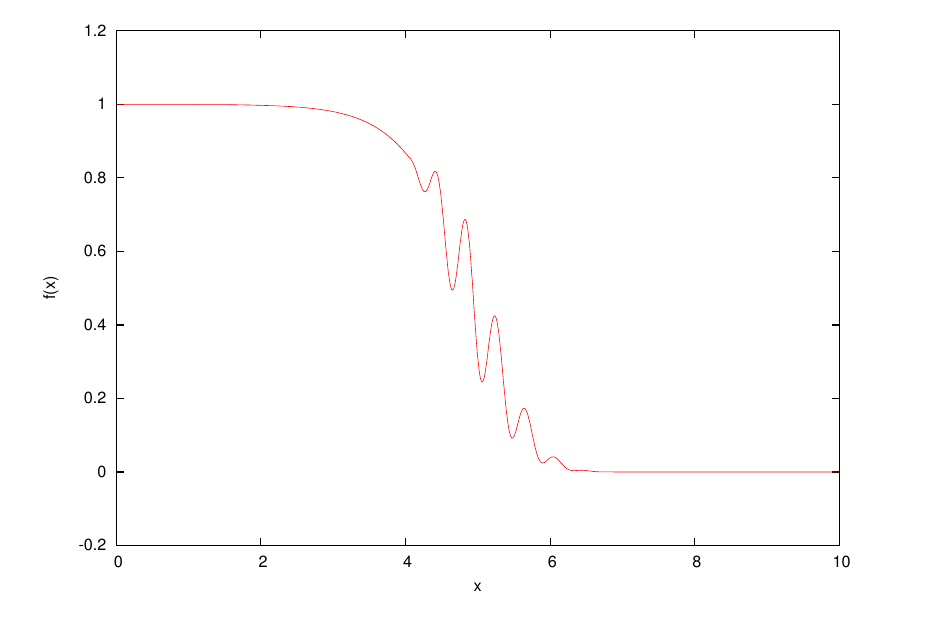
\includegraphics[width=10cm]{./Figures/20170227-nc-adaptive-quadrature.png}
  \label{fig:ninc-nc-singularity-adaptive-quadrature}
%
%  \small{Source: PBOC.}
\end{figure}

\subsection{克伦肖——柯蒂斯法则}
\label{sec:ninc-cc-rules}

如前文所述,牛顿——柯蒂斯求积法则(第\ref{sec:nint-nc-rule}节)的近似误差随着分段数$N$的衰减速度并不够令人满意;若是尝试利用更高阶多项式被积方程做近似,还会受到龙格现象的干扰。因此在实际应用中,常常并不会直接使用牛顿——柯蒂斯法则。一个更好的方案是克伦肖——柯蒂斯求积法则(Clenshaw-Curtis Rule)\index{Clenshaw-Curtis Rule \dotfill 克伦肖——柯蒂斯求积法则}。
在了解傅里叶分析(第\ref{sec:fourier-analysis}节)的基本要点之后,我们可以对这个法则有大致介绍。


\section{傅里叶分析}
\label{sec:fourier-analysis}

我们可以这样理解分析(analysis):将研究对象分解成小块来分别研究。那么我们可以这样理解傅里叶分析(Fourier analysis):将研究对象(方程)分解为小块,即不同的弦波(sinosoids),每个小快都以有限的速度变化。例如这个方程
\begin{equation*}
  f(t) = 3 \cos 2 \pi t + 19 \sin 4\pi t - 0.14 \cos 7 \pi t,
\end{equation*}
可以分解为
\begin{equation*}
  \begin{split}
    f(t) & = 3 A + 19 B - 0.14 C,
  \end{split}
\end{equation*}
其中$A,B,C$分别表示角频率(angular frequency)\index{angular frequency \dotfill 角频率}为$2 \pi, 4 \pi, 7 \pi$的弦波。

但对于这样的方程
\begin{equation*}
\begin{split}
    f(t) &  = \exp \left( - \alpha \left| t \right| \right), \\
    f(t) & = \begin{cases}
    1, & \left| t \right| < 1 \\
    2, & \left| t \right| > 1
    \end{cases},
\end{split}
\end{equation*}
甚至更复杂一些的方程,该如何做傅里叶分析?

在开始正式介绍之前,有必要做一些简单的概念界定,见表\ref{tab:fourier-analysis-definition}。

\begin{table}[htbp]
\caption{傅里叶分析的常见概念界定}
%\begin{flushleft}
\begin{tabular}{|l|c|c|}
\hline
 & 连续方程 $f(t)$ & 离散方程 $f_{n} \equiv f \left( n \Delta t \right), n \in \mathcal{Z}$\\ \hline
无限域 $- \infty < t < \infty$  & 傅里叶变换 (Fourier transform) \index{Fourier transform! \dotfill 傅里叶变换}& 半离散傅里叶变换 (Semidiscrete Fourier transform)\index{Fourier transform!Semidiscrete \dotfill 半离散傅里叶变换} \\ \hline
有限域 $- \frac{T}{2} < t < \frac{T}{2}$ & 傅里叶级数 (Fourier seires)\index{Fourier series \dotfill 傅里叶级数} & 离散傅里叶变换 (Discrete Fourier transform)\index{Fourier transform!Discrete \dotfill 离散傅里叶变换} \\ \hline
\end{tabular}
%\end{flushleft}
\label{tab:fourier-analysis-definition}
\end{table}

\subsection{傅里叶变换}
\label{sec:fourier-transform}
我们先从表\ref{tab:fourier-analysis-definition}左上角的傅里叶变换开始介绍,即连续方程$f(t)$在无限时间区间$(-\infty, \infty)$的求积问题。
\begin{equation}
  \label{sec:fourier-transform-definition}
  \tilde{f} \left( \omega \right) =
  \frac{1}{2 \pi} \int_{-\infty}^{\infty}
  \exp \left( - i \omega t \right) f(t) \, \mathrm{d} t,
\end{equation}
其中$f \left( \omega \right)$是一个关于频率$\omega$的方程,方程形式反映了在频率域$\omega$中表现出的非线性(指数)强烈程度。

现在基于傅里叶变换式\eqref{sec:fourier-transform-definition}来回顾前面的问题:如何将方程$E_{\alpha}(t) = \exp \left( - \alpha \left| t \right| \right)$分解为一组弦波组合的形式?其基本思路是,通过将所有关于频率$\omega$的弦波曲线加总来重写原方程$\exp \left( - \alpha \left| t \right| \right)$,某一弦波的频率越大,振幅(amplitude)。
\begin{equation*}
  \begin{split}
    \widetilde{E}_{\alpha} \left( \omega \right)
    & = \frac{1}{2 \pi}
    \int_{-\infty}^{\infty} \exp \left( - i \omega t \right) \exp \left( - \alpha \left| t \right| \right) \, \mathrm{d} t \\
    & = \frac{1}{2 \pi} \left\{
    \int_{-\infty}^{0} \exp \left[ \left( - i \omega + \alpha \right) t \right] \, \mathrm{d} t
    + \int_{0}^{\infty} \exp \left[ \left( - i \omega - \alpha \right) t \right]
    \right\} \\
    & = \frac{1}{2 \pi}
    \left[
    \frac{1}{\alpha - i \omega}
    - \frac{1}{\alpha + i \omega}
    \right] \\
    & = \frac{\alpha}{\pi \left( \alpha^{2} + \omega^{2} \right)},
  \end{split}
\end{equation*}
注意,这里所说的``频率"$\omega$越大或越小,是相对于参数$\alpha$而言的:$\alpha$越大,指数方程$E_{\alpha}(t)$越快衰减至$0$,我们就越需要增加$\widetilde{E}_{\alpha}(\omega)$的振幅,利用更高振幅的弦波来近似原方程。下面将作进一步说明。

\subsubsection{一些概念}
\begin{equation*}
  y = A \sin \left( B x + c \right) + D,
\end{equation*}
其中
\begin{itemize}
  \item $A$表示振幅,
  \item $\frac{B}{2 \pi}$表示周期,$\text{频率} = \frac{1}{\text{周期}}$,
  \item $- \frac{C}{B}$表示相位的(水平)移动,
  \item $D$表示相位的(垂直)移动。
\end{itemize}

\begin{figure}[htbp]
   \caption{傅里叶变换}
  \centering
  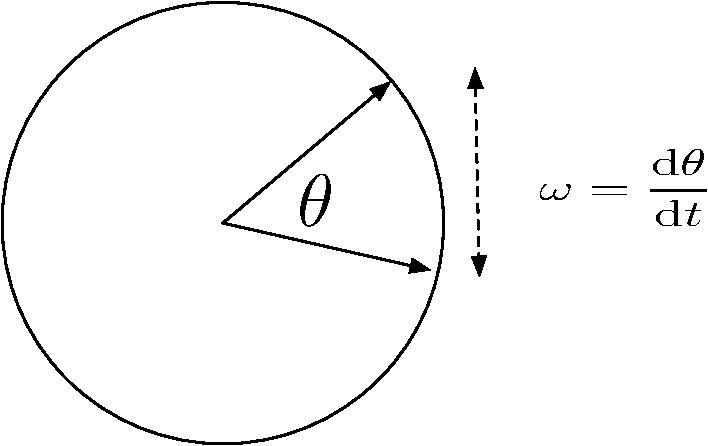
\includegraphics[width=8cm]{./Figures/20180302-frequencies-etc.pdf}
  \label{fig:fourier-basic-concepts}
%
%  \small{Source: PBOC.}
\end{figure}
图\ref{fig:fourier-basic-concepts}中
\begin{itemize}
  \item $\omega = \frac{2 \pi}{T} = 2 \pi \nu = %\frac{\nu}{r}
  = \frac{\mathrm{d} s}{\mathrm{d} t} \cdot \frac{1}{r} = \frac{\mathrm{d} \theta}{\mathrm{d} t}$
  \item $\omega$,角频率(angular frequency)\index{angular frequency \dotfill 角频率},是对物体旋转速度快慢的度量,单位如弧度/秒(radian/second)。
  \item $T$,周期,单位如秒。
  \item $\nu$,线频率(linear frequncy),单位如赫兹(Hertz),$1 Hertz = 1\text{次/秒}$。
  %\item 绕轴旋转的线速度,单位如米/秒。
  \item 旋转的半径,单位如米。
\end{itemize}

\subsubsection{线频率和角频率}
\label{sec:fourier-frequency-linear-angular}
对于一个给定的弦波方程如$\sin \omega t$或$\exp \left[ - i \omega t\right]$等,严格说来我们需要将其中的频率$\omega$理解为角频率$\omega$(angular frequency)\index{angular frequency \dotfill 角频率},表示相角旋转速度的快慢,单位如角每秒(radian per second)。线频率(linear frequency)可写为\index{linear frequency \dotfill 线频率}$\nu = \frac{\omega}{2 \pi}$,表示这一过程自我重复的频率,单位如赫兹。例如,一个钟摆4秒钟转一圈,那么
\begin{itemize}
  \item 周期$T=4$,
  \item 角频率$\omega = \frac{2 \pi}{T} = \frac{\pi}{2} \approx 1.57 Rad/s$,
  \item 线频率$\nu = \frac{1}{T} = 0.25 Hz$。
\end{itemize}

\subsubsection{域}
\label{sec:fourier-domains}

\eqref{sec:fourier-transform-definition}对原方程$f(t)$作傅里叶变换,生成近似方程$\tilde{f}(\omega)$,二者等价但处于不同的域中。$f(t)$的解释变量是(时间)$t$,$\tilde{f}(\omega)$的解释变量是频率$\omega$,从这个角度可以说,$f(t)$是在时间域中,$\tilde{f}(\omega)$是在频率域中。

福利也分析也可用于原方程$f$的解释变量不是时间的情况,例如可以是方位$x$,对应的傅里叶变换处于空间频率$k$中,有时也称波数(wavenumber)\index{wavenumber \dotfill 波数}。更多例子见下表。

\begin{table}[htbp]
\caption{原方程域和傅里叶变换方程域}
%\begin{flushleft}
\begin{tabular}{|l|cccc|}
\hline
& 原变量 & 原域 & 傅里叶变量& 傅里叶域 \\ \hline
信号处理 & 时间$t$ & 时间域 & 频率$\omega$ & 频率域 \\
光学 & 方位$x$ & 实空间 & 波数$k$ & $k$空间 \\
量子力学 & 方位$x$ & 方位空间 & 动量(momentum)$p$ & 动量空间 \\
固体物理学 & 点阵向量$L$ & 实空间 & 布洛赫向量(Bloch vector) $k$ & 晶体动量空间(crystal momentum space)
\\ \hline
\end{tabular}
%\end{flushleft}
\label{tab:fourier-domain-definition}
\end{table}

\subsubsection{单位}
实际研究过程中需要牢记$f(t)$和$\tilde{f}(\omega)$的单位不同。以\eqref{sec:fourier-transform-definition}为例,RHS中有$\mathrm{d} t$,LHS中没有。因此
\begin{equation*}
    \tilde{f}\text{的单位} = f\text{的单位} \times \text{时间} = \frac{f\text{的单位}}{\text{频率}},
\end{equation*}
如果$f$的单位是伏特(Volt),那么$\tilde{f}$的单位是伏特秒,或者伏特每赫兹。

\subsubsection{傅里叶变换的性质}
\label{sec:fourier-properties}
由定义\eqref{sec:fourier-transform-definition}可得,傅里叶变换具有如下性质,我们将分别作说明。
\begin{itemize}
  \item 导数的傅里叶变换
  \item 傅里叶变换的导数
  \item 实值方程的傅里叶变换
\end{itemize}

\textit{导数的傅里叶变换}。对于某一给定方程$f(x)$,如果我们可以求得其傅里叶变换$\tilde{f}(k)$,那么$f(x)$的导数也很容易写出。首先写出$f(t)$的傅里叶综合表达式(Fourier synthesis equation)\todo{做一个reference}
\begin{equation*}
  f(x) = \int_{-\infty}^{\infty} \tilde{f}(k) \exp \left( i k x \right) \, \mathrm{d} k,
\end{equation*}
两侧同时对$x$求导
\begin{equation*}
  \frac{\mathrm{d}}{\mathrm{d} x}f(x)
  = \int_{-\infty}^{\infty} i k \tilde{f}(k) \exp \left( i k x \right) \, \mathrm{d} k,
\end{equation*}
上式的RHS是对$\left( i k \widetilde{f} (k) \right)$的逆傅里叶变换(Definition \ref{definition:fourier-transformation});因此可以将RHS看作是$\frac{\mathrm{d}}{\mathrm{d} x}f(x)$的傅里叶变换,即
\begin{equation}
  \label{eq:fourier-derivative-ft-eq}
  \mathcal{F}\left[ f(x) \right]
  = \tilde{f}(k) \Rightarrow \mathcal{F}
  \left[
  \frac{\mathrm{d}}{\mathrm{d} x}f \left( x \right)
  \right] = i k \tilde{f}(k).
\end{equation}

也可以重复上述过程求解高阶导数,如
\begin{equation}
  \label{eq:fourier-derivative-ft-eq-higher}
  \mathcal{F} \left[ f(x) \right] = \tilde{f}(k)
  \Rightarrow
  \mathcal{F} \left[ \frac{\mathrm{d}}{\mathrm{d} x} f(x) \right]
  = i k \tilde{f} (k)
  \Rightarrow
  \mathcal{F}
  \left[
  \frac{\mathrm{d}^{2}f}{\mathrm{d} x^2} \right]
  = - k^{2} \tilde{f}(k).
\end{equation}

\textit{傅里叶变换的导数}。
类似地,对傅里叶变换\eqref{sec:fourier-transform-definition}
\begin{equation*}
  \tilde{f} \left( k \right) =
  \frac{1}{2 \pi} \int_{-\infty}^{\infty}
  \exp \left( - i k x \right) f(x) \, \mathrm{d} x
\end{equation*}
两侧求$k$的导数有
\begin{equation*}
  \frac{\mathrm{d}}{\mathrm{d} k} \tilde{f}(k)
  = \int_{-\infty}^{\infty} - i x f(x) \exp \left( - i k x \right) \, \mathrm{d} x,
\end{equation*}
可见$\frac{\mathrm{d}}{\mathrm{d} k} \tilde{f}(k)$可以看成是方程$x \cdot f(x)$的傅里叶变换。因此有
\begin{equation}
  \label{eq:fourier-ft-derivative-eq}
  \mathcal{F}\left[ f(x) \right] = \tilde{f}(k)
  \Rightarrow \mathcal{F} \left[ x f(x) \right]
  = i \frac{\mathrm{d}}{\mathrm{d} k }\tilde{f}(k).
\end{equation}

不难看出,\eqref{eq:fourier-derivative-ft-eq} 和\eqref{eq:fourier-ft-derivative-eq}等价。

\textit{实值方程的傅里叶变换}。
如果$f(x)$是一个实值方程,那么它对应的傅里叶变换$\tilde{f}(k)$中所含有的信息中,相对于$k<0$的部分就是冗余信息:$\tilde{f}\left(k \right) \big|_{k <0 }$的信息可由$\tilde{f}\left(k \right) \big|_{k > 0}$的部分而获得。以定义式为例,对于$k<0$的情况下有
\begin{equation*}
\tilde{f}\left( - k \right) = \frac{1}{2 \pi} \int_{- \infty}^{\infty} f(x) \exp \left( i k x \right) \, \mathrm{d} x,
\end{equation*}
由于假定$f(x)$是一个实值方程,进一步可得
\begin{equation*}
%  \label{eq:fourier-real-valued-func}
  \tilde{f}(-k) =
  \left[
  \frac{1}{2 \pi} \int_{- \infty}^{\infty} f(x) \exp \left( - i k x \right) \, \mathrm{d} x
  \right]^{*}
  = \tilde{f}^{*} (k).
\end{equation*}


\subsection{脉冲方程的傅里叶变换}
\label{sec:fourier-function-types}
介绍几种常见的傅里叶变换。

\subsubsection{洛伦兹变换}
\label{sec:fourier-lorentzian-transformation}
以前文提到的方程为例
\begin{equation}
  \label{eq:fourier-lorentzian}
  E_{\alpha} \left( x \right) = \exp \left( - \alpha \left| x \right| \right), \quad \widetilde{E}_{\alpha} \left( k
  \right) = \frac{
  \alpha
  }{
  \pi \left( \alpha^{2} + k^{2} \right)
  }.
\end{equation}

$E_{\alpha} \left( x \right)$和$\widetilde{E}_{\alpha} \left( k
\right)$都可以被看作是某种脉冲方程(pulse functions):它们都在初始点$x_{0} ,k_{0}$处附近有最大值,又随着$x \rightarrow \infty$或$k \rightarrow \infty$而逐渐降低直至$0$,称为洛伦兹变换(Lorentzian function)\index{Lorentzian function \dotfill 洛伦兹方程}。两个方程的宽度均与参数$\alpha$有关,但影响方向相反:$\alpha$的值越大,实空间中的脉冲越弱、宽度越窄,傅里叶空间中的脉冲越强、宽度越宽,如图\ref{fig:fourier-lorentzian-trans}所示。
\begin{figure}[htbp]
   \caption{洛伦兹方程$(\alpha = 2)$}
  \centering
  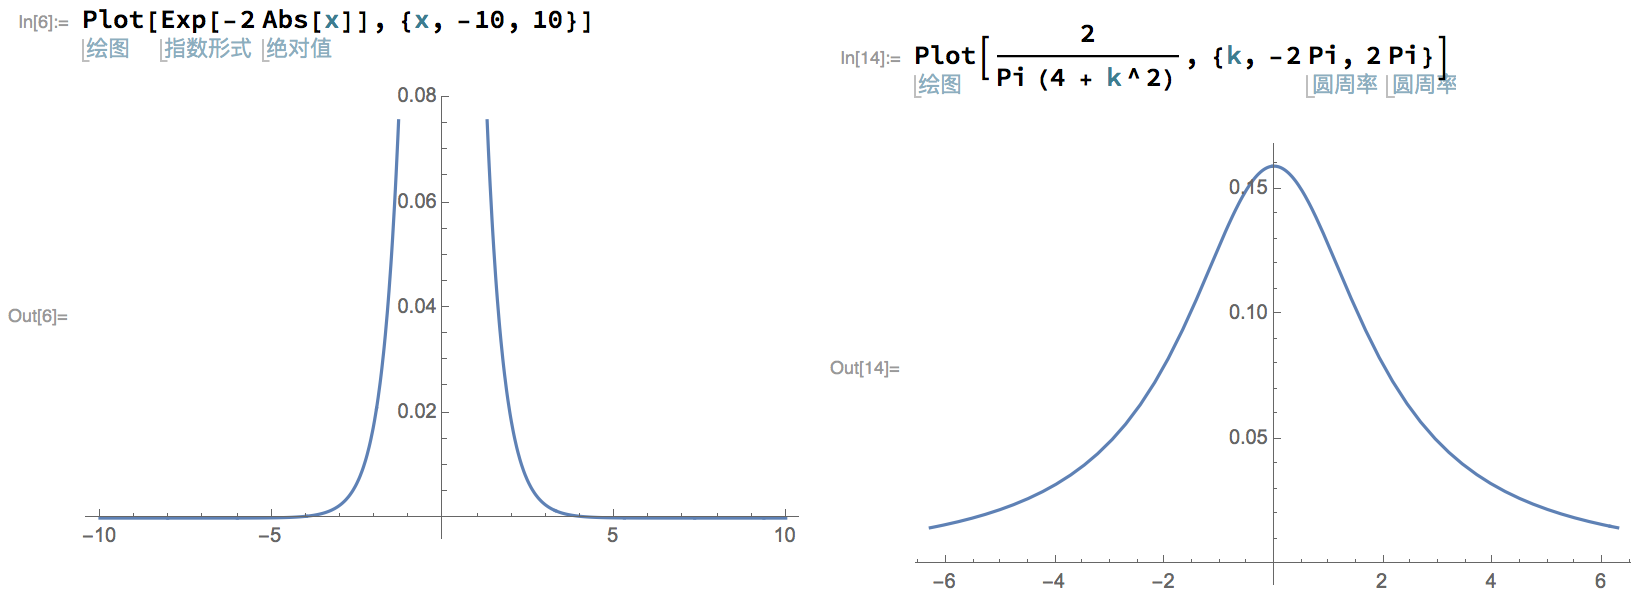
\includegraphics[width=14cm]{./Figures/20180304-lorentzian-example.png}
  \label{fig:fourier-lorentzian-trans}
%
%  \small{Source: PBOC.}
\end{figure}

我们将脉冲的一个半峰全宽(full width at half maximum, FWHM)\index{full width at half maximum(FWHM) \dotfill 半峰全宽}定定义为,在方程的一个周期中,前后两个方程值等于一个峰值一半的点之间的距离。根据这个定义,$E_{\alpha}(x)$的峰值为$1(x=0)$,并且在$x \pm (\ln 2) / \alpha$时,值为峰值的一半,因此有
\begin{equation}
  \label{eq:fourier-lorentzian-fwhm-e}
  FWHM \left[ E_{\alpha} (x) \right] = \frac{2 \ln 2}{\alpha},
  \end{equation}
$\widetilde{E}_{\alpha}(k)$的峰值为$\frac{1}{\pi \alpha} (k = 0)$,在$k = \pm \alpha$时,值为峰值的一半,
\begin{equation}
    \label{eq:fourier-lorentzian-fwhm-tilde-e}
    FWHM \left[ \widetilde{E}_{\alpha}(k) \right] = 2 \alpha.
\end{equation}

\eqref{eq:fourier-lorentzian-fwhm-e}和\eqref{eq:fourier-lorentzian-fwhm-tilde-e}联立有
\begin{equation}
  \label{eq:fourier-lorentzian-fwhm-product}
  FWHM \left[ E_{\alpha} (x) \right] \cdot FWHM \left[ \widetilde{E}_{\alpha}(k) \right] = 4 \ln 2,
\end{equation}
注意:单个原方程及洛伦兹变换方程的FWHM与$\alpha$有关;两个$FWHM$的乘积则与$\alpha$无关:所有洛伦兹脉冲方程族$\left\{ E_{\alpha}(t) \right\}$都具有这样的特征。

\subsubsection{高斯变换}
\label{sec:fourier-gaussian}
设一个宽度为$\sigma$的高斯方程(Gaussian function)\index{Gaussian function \dotfill 高斯方程}
\begin{equation*}
  G_{\sigma}(x) = \exp \left( - \frac{x^{2}}{\sigma^{2}}\right),
\end{equation*}
那么其傅里叶变换
\begin{equation*}
  \begin{split}
    \widetilde{G}_{\sigma} \left( k \right)
    & = \frac{1}{2 \pi}
    \int_{-\infty}^{\infty} \exp \left( - i k x \right)
    G_{\sigma} \left( x \right) \, \mathrm{d} x \\
    & = \frac{1}{2 \pi}
    \int_{-\infty}^{\infty}
    \underbrace{
    \exp
    \left(
    - i k x - \frac{x^{2}}{\sigma^{2}}
    \right)
    }_{\eqqcolon \mathcal{A} }
    \, \mathrm{d} x,
  \end{split}
\end{equation*}
RHS的被积方程
\begin{equation*}
  \begin{split}
    \mathcal{A} & = \frac{1}{\sigma^{2}}
    \left( x^{2} + i k x \sigma^{2} \right) \\
    & = \frac{1}{\sigma^{2}}
    \left(
    x + \frac{1}{2} i k \sigma^{2}
    \right)^{2} + \frac{1}{4} k^{2} \sigma^{2} \\
    & = \frac{1}{2 \pi} \exp \left( - \frac{1}{4} k^{2} \sigma^{2} \right)
    \underbrace{
    \int_{-\infty}^{\infty} \exp
    \left[
    - \frac{1}{\sigma^{2}}
    \left( x + \frac{1}{2} i k \sigma^{2} \right)^{2}
    \right] \, \mathrm{d} x
    }_{= \sigma \cdot \sqrt{\pi}} \\
    & = \frac{\sigma}{2 \sqrt{\pi}} \exp \left( - \frac{1} {4} k^{2} \sigma^{2} \right),
  \end{split}
\end{equation*}

可见$\widetilde{G}_{\sigma}(k)$也是一个$k$空间中的高斯方程,其宽度与原方程$G_{\sigma}(x)$的宽度成等比例
\begin{equation*}
  \widetilde{G}_{\sigma} \propto \exp \left( - \frac{k^{2}}{\tilde{\sigma}^{2}} \right) = G_{\tilde{\sigma}} \left( k \right), \quad \tilde{\sigma} \equiv \frac{2}{\sigma}.
\end{equation*}

此外
\begin{equation}
    \label{eq:fourier-gaussian-fwhm-product}
  \begin{split}
    FWHM \left[ G_{\sigma} \left( x \right) \right]
    & = 2 \sqrt{ \ln 2} \sigma, \\
    FWHM \left[ G_{\sigma} \left( x \right) \right] \cdot FWHM \left[ \widetilde{G}_{\sigma} \left( x \right) \right]
    = \left( 2 \sqrt{\ln 2} \sigma \right) \cdot
    \left( \frac{4 \sqrt{\ln 2}}{\sigma}\right) = 8 \left( \ln 2\right)^{2},
  \end{split}
\end{equation}
可见单个原高斯方程及高斯变换方程的FWHM与$\alpha$有关;两个$FWHM$的乘积则与$\alpha$无关:所有高斯脉冲方程族$\left\{ G_{\sigma}(x) \right\}$都具有这样的特征。

\subsection{非脉冲方程的傅里叶变换}
\label{sec:fourier-non-pulse-functions}
洛伦兹变换和高斯变换都属于脉冲方程,特点是初始点附近有峰值,随着$x$($k$)逐渐增大而慢慢回落至$0$。如何求得非脉冲方程的傅里叶变换,如$f(x) = 1, \, f(x)=x, $或$f(x) = x^{2}$呢?

一种求解思路是,考虑\eqref{eq:fourier-lorentzian}在$\lim_{\alpha \rightarrow 0}$时的情况,实值方程趋近于$1$
\begin{equation*}
  \lim_{\alpha \rightarrow 0} E_{\alpha}(x) \rightarrow 1.
\end{equation*}

而它的洛伦兹变换$\widetilde{E}_{\alpha}(k)$的求解则较为复杂,第一它的宽度变窄了$FWHM \widetilde{E}_{\alpha} = 2 \alpha$;第二它的高度变高了$\widetilde{E}_{\alpha} \left( 0 \right) = \frac{1}{\pi \alpha}$。随着$\alpha \rightarrow 0$的极限情况出现,$\lim_{\alpha \rightarrow 0} \widetilde{E}_{\alpha}(k)$变得极窄、极高,就成为狄拉克方程(dirac delta function) \index{dirac delta function \dotfill 狄拉克方程}
\begin{equation}
  \label{eq:fourier-non-pulse-dirac}
  \lim_{\alpha \rightarrow 0} \widetilde{E}_{\alpha}(k) = \lim_{\alpha \rightarrow 0} \frac{
  \alpha
  }{\pi \left( \alpha^{2} + k^{2} \right)}
  \equiv \delta (k) = \begin{cases}
  + \infty & k = 0, \\
  0 & k \neq 0,
\end{cases} \quad \Rightarrow \int_{- \infty}^{\infty} \delta (k) \, \mathrm{d} k = 1.
\end{equation}

对应地,非脉冲方程$f(x) =1$的傅里叶变换可以写作
\begin{equation}
  \label{eq:fourier-non-pulse-ftran-1}
  f(x) \equiv 1 \Rightarrow \tilde{f}(k) = \delta(k),
\end{equation}
可以这么理解:$f(x) \equiv 1$是一个频率为$0$的弦波。对$f(x)$做傅里叶转换,分解为若干弦波之和,在这一系列弦波中,我们将除了第一条(对应频率为$0$)之外的其他全部弦波曲线的系数值均设为$0$。

在此基础上,利用\eqref{eq:fourier-non-pulse-ftran-1}和\eqref{eq:fourier-ft-derivative-eq},进一步可得到另外两个非脉冲方程的傅里叶变换
\begin{align}
  \label{eq:fourier-non-pulse-ftran-x1}
  f(x) = x \quad \Rightarrow \tilde{f}(k) = i \delta^{'}(k), \\
  \label{eq:fourier-non-pulse-ftran-x2}
  f(x) = x^{2} \quad \Rightarrow \tilde{f}(k) = - \delta^{''}(k),
\end{align}

其中$\delta'(k)$是狄拉克方程的导数,基于\eqref{eq:fourier-non-pulse-dirac}用分部积分法有
\begin{equation*}
  \int f(u) \delta^{'}(u) \mathrm{d} u =
  - \int f^{'}(u) \delta(u) \, \mathrm{d} u = - f^{'}(u),
\end{equation*}
可见$\delta'$可以被看做是和$\delta$相近的方程,二者只有一点不同:利用分部求积计算$\delta'$时产生了$- f'(0)$的变化,而$\delta$只产生$-f$的变化。

需要指出的是,对非脉冲方程的傅里叶变换如\eqref{eq:fourier-non-pulse-ftran-1}、\eqref{eq:fourier-non-pulse-ftran-x1}、\eqref{eq:fourier-non-pulse-ftran-x2},都不算是``好''的方程——它们甚至不是方程,而只是分布(比如狄拉克方程单独出现往往没有实际意义,它更多是与其他定义良好的方程配对出现在积分式中):这么说是因为$f(x)= \left\{ 1, x, x^{2} \right\} \notin L^{1}$,即它们不满足$\int_{-\infty}^{\infty} \left| f(x) \right| \, \mathrm{d}x < \infty$。
\footnote{$L^{1}$表示勒贝格空间,见第\eqref{sec:lesbegue-space}节。}
因此,\eqref{eq:fourier-non-pulse-ftran-x2}等傅里叶变换,往往更适合以算子的形式出现。

\subsection{原方程的平滑和傅里叶变换方程的衰减}
\label{sec:fourier-smoothness-decay}
通过前面的分析不难总结出一个一般规律:原方程$f(t)$越是(口语意义上的)不``平滑'',即随着解释变量$t$的变动而剧烈变动,其傅里叶变换$\tilde{f} \left( \omega \right)$随着$\omega$的衰减(decay)速度就越慢。反之亦然:$f(t)$越平滑,$\tilde{f} \left( \omega \right)$的衰减就越快。可以将$f(t)$的平滑特性表现为$f$的连续性和导数:
\begin{theorem}[佩利——维纳诸定理]
  \label{theorem:paley-wiener-theorems}
  如果$f(t)$和它的前$p-1$个导数都是连续的,但第$p$个导数是不连续的,并且变差有界(bounded variation),那么$\tilde{f}(\omega)$的衰减速度不低于$\left| \omega \right|^{- \left( p + 1 \right)} \big|_{\omega \rightarrow \infty}$。  这称为佩利——维纳诸定理(Paley-Wiener theorems)\index{Paley-Wiener theorems \dotfill 佩利——维纳诸定理}。
\end{theorem}
\begin{proof}
  略。可参考如\cite[Sec. VI.4]{Yosida:1978ul},\cite[Theorem 4.1.2]{Agranovich:2015cv}。
\end{proof}

  尤其是,若$f(t) \in C^{\infty}$,\footnote{空间$C^{\infty}$中的方程连续,所有导数也都连续,可参考第\ref{sec:spaces-c}节。}那么在$\omega$值较大时,$\tilde{f}(\omega)$的衰减速度比任何多项式都快。这样的方程包括诸如$\exp \left( - \omega \right)$,$\exp \left( - \sqrt{\omega} \right)$,$\exp \left( - \omega^{2} \right)$等。

举例如洛伦兹方程$\exp \left( - \alpha \left| t \right| \right)$连续,但其一阶导数不连续,表现为在$t=0$处有跳跃,如图\ref{fig:fourier-lorentzian-trans}左侧。因此$p=1$。对应地,我们会看到它的傅里叶变换以等比于$\omega^{-2}$的速度衰减(当$\omega$的值较大时)。

再比如,方程$\exp \left( - \frac{t^{2}}{\sigma^{2}} \right) \in C^{\infty}$,那么其傅里叶变换$\widetilde{F} = \exp \left( - \frac{1}{4} \sigma^{2} \omega^{2} \right)$的衰减速度快于任意多项式。

\subsection{傅里叶级数}
\label{sec:fourier-seires}
现在来看表\ref{tab:fourier-analysis-definition}左下一栏,对应有限空间中连续方程$f(t)$的傅里叶分析,称为傅里叶级数。

假设$f(t)$是个关于$T$的周期方程(periodic function)\index{periodic function \dotfill 周期方程},即每隔$T$单位时间(秒,分,小时,天等)就自我重复一遍:
\begin{equation*}
  f(t+T) \equiv f(t), \quad \forall t.
\end{equation*}

假定$f(t)$符合傅里叶分析的条件,对应傅里叶变换
\begin{equation}
  \label{eq:fourier-series-def}
  \tilde{f}(\omega) = \frac{1}{2 \pi} \int_{-\infty}^{\infty}
  \exp \left( - i \omega t \right) f(t) \, \mathrm{d} \omega,
\end{equation}
随着角频率$\omega$和基准频率(base frequency) $
\omega_{0}=\frac{2 \pi}{T}$的关系不同,需要分两种情况来分析:
\begin{enumerate}
  \item $\omega$是$\omega_{0}$的整数倍。

  那么\eqref{eq:fourier-series-def}中的被积方程周期为$T$,每个宽度为$T$的子区间对总积分的作用相同,并且由于这样的子区间有无数个,我们有$\tilde{f} \left( \omega \right) = \infty$。
  \item $\omega$是$\omega_{0}$的整数倍。

  那么\eqref{eq:fourier-series-def}中的被积方程不是一个周期方程。我们可以将$f(t)$理解为两部分:一部分是$f(t)$,这是一个关于$T$的周期方程,另一部分是$\exp \left( - i \omega t \right)$,它只有在某些特定的时期才是周期方程,这些特定的时期是指不等于$T$的整数倍的时期。两部分的乘积导致被积方程不是一个周期方程。

  每个宽度为$T$的子区间都给总积分值产生同等程度的影响,但影响的大小(phase,相)是随机的。各个随机相的影响加总后相互抵消,$\tilde{f}(\omega) =0$。
\end{enumerate}

将上述两种情况汇总可见,在$f(t)$是一个周期方程的前提下
\begin{equation*}
  \tilde{f}(\omega) =
  \begin{cases}
    \infty, & \omega\text{是}\omega_{0}\text{的整数倍},\\
    0, & \text{否则}.
  \end{cases}
\end{equation*}

我们可以用三种数学形式将上式表达出来:
\begin{enumerate}
  \item 利用狄拉克方程,可将$T$-周期方程的傅里叶变换表示为
  \begin{equation}
    \label{eq:fourier-series-dirac}
    \tilde{f}(\omega) = \sum_{\nu = - \infty}^{\infty}
    \tilde{f}_{\nu} \cdot \delta \left( \omega - \nu \omega_{0} \right), \quad \omega_{0} \equiv \frac{2 \pi}{T}, \, \nu \in \mathcal{Z}.
  \end{equation}
  \item 对$T$-周期方程$f(t)$的傅里叶分解,只包括那些频率为$\omega_{\nu}$的弦波曲线,满足$\omega_{\nu} = \nu \cdot \omega_{0} = \frac{2 \nu \pi}{T}, \, \nu \in \mathcal{Z}$,记作
  \begin{equation}
    \label{eq:fourier-series-exponential}
    f(t) = \sum_{\nu \in \mathcal{Z}} \tilde{f}_{\nu} \cdot \exp \left( i \nu \omega_{0} t \right), \quad \omega_{0} = \frac{2 \nu \pi}{T}, \, \nu \in \mathcal{Z},
  \end{equation}
  我们又将\eqref{eq:fourier-series-exponential}称为傅里叶级数(Fourier series)\index{Fourier series \dotfill 傅里叶}的表达形式之一:复杂指数表达形式。

  \item 除此之外,也可以将傅里叶级数表达为另一种形式,即一组正弦函数和一组余弦函数之和
  \begin{equation}
    \label{eq:fourier-series-sin}
    f(t) = \sum_{\nu = 0}^{\infty} \tilde{a}_{\nu} \cdot \cos \left( \nu \omega_{0} t \right)
    + \sum_{\nu = 1}^{\infty} \tilde{b}_{\nu} \cdot \sin \left( \nu \omega_{0} t \right), \quad \nu \in \mathcal{Z}^{+}.
  \end{equation}
\end{enumerate}

\subsubsection{两种表达形式的比较}
  \eqref{eq:fourier-series-sin}中的$\nu$需要取正整数;\eqref{eq:fourier-series-exponential}则正负均可。除此而外,指数形式\eqref{eq:fourier-series-exponential}和弦波形式\eqref{eq:fourier-series-sin}等价,可以被看作是同一个$T$-周期方程$f(t)$的傅里叶级数分解。

来看两组系数$\left\{ \tilde{a}_{\nu}, \tilde{b}_{\nu} \right\}_{\nu \in \mathcal{Z}^{+}}$和$\left\{ \tilde{f}_{\nu} \right\}_{\nu \in \mathcal{Z}}$之间的关系。已知复杂指数$\exp \left( i \nu \omega_{0} t \right)$可表示为关于正弦和余弦函数的方程
\begin{equation}
  \label{eq:fourier-series-complex-expo}
  \exp \left( i \nu \omega_{0} t \right) = \cos \left( \nu \omega_{0} t \right) + i \sin \left( \nu \omega_{0} t \right),
\end{equation}
以及三角函数关系:余弦函数是偶函数,正弦函数是奇函数
\begin{equation}
  \label{eq:fourier-cos-even-sin-odd}
  \cos \left( - A \right) = \cos \left( A \right), \quad \sin \left( - A \right) = - \sin \left( A \right),
\end{equation}

结合\eqref{eq:fourier-series-exponential}-\eqref{eq:fourier-cos-even-sin-odd}可得
\begin{equation}
  \label{eq:fourier-series-representation-relation-coef}
  \begin{split}
    \tilde{a}_{0} & = \tilde{f}_{0}, \\
    \tilde{a}_{\nu} & = \left( \tilde{f}_{\nu} + \tilde{f}_{- \nu} \right), \quad \nu > 0, \\
    \tilde{b}_{\nu} & = i \left( \tilde{f}_{\nu} - \tilde{f}_{- \nu} \right), \quad \nu > 0,
  \end{split}
\end{equation}

或者反过来
\begin{equation}
  \label{eq:fourier-series-representation-relation-coeff}
  \tilde{f}_{\nu} =
  \begin{cases}
  \frac{1}{2} \left( \tilde{a}_{\nu} + i \tilde{b}_{\nu} \right), & \nu < 0, \\
  \tilde{a}_{0}, & \nu = 0, \\
  \frac{1}{2} \left( \tilde{a}_{\nu} - i \tilde{b}_{\nu} \right), & \nu > 0.
  \end{cases}
\end{equation}

比较两种表达式形式:复杂指数形式\eqref{eq:fourier-series-exponential}和正弦余弦形式\eqref{eq:fourier-series-sin}:
\begin{enumerate}
  \item \eqref{eq:fourier-series-sin}的好处在于
  \begin{enumerate}
    \item 若$T$-周期$f(t)$是实值方程,那么其傅里叶变换系数$\left\{ \tilde{a}_{\nu}, \tilde{b}_{\nu} \right\}_{\nu \in \mathcal{Z}^{+}}$也都是实值系数,从而无需考虑复数的情况。
    \item 结合具体$f(t)$的奇偶性,可以作灵活调整,从而简化后续的计算工作。例如若$f(t)$是偶函数,那么它的傅里叶变换只包含余弦项;全部正弦项都消失了,因此无需计算$\tilde{b}_{\nu}$。
  \end{enumerate}
  \item \eqref{eq:fourier-series-exponential}的好处在于
  \begin{enumerate}
    \item 只需计算一组系数$\left\{ \tilde{f}_{\nu} \right\}_{\nu \in \mathcal{Z}}$,而非两组系数$\left\{ \tilde{a}_{\nu}, \tilde{b}_{\nu} \right\}_{\nu \in \mathcal{Z}^{+}}$。
    \item 指数形式傅里叶级数的推算公式\eqref{eq:fourier-series-exponential}更直观和易于理解。
    \item 求导更容易。事实上对\eqref{eq:fourier-series-exponential}求导后生成的傅里叶级数仍然是\eqref{eq:fourier-series-exponential},只是原来的系数$\left\{ \tilde{f}_{\nu} \right\}_{\nu \in \mathcal{Z}}$
    现在变成了$\left\{ i \omega_{0} \tilde{f}_{\nu} \right\}_{\nu \in \mathcal{Z}}$。反观\eqref{eq:fourier-series-sin},求导操作更为复杂。
  \end{enumerate}
\end{enumerate}

基于上述考虑,在大多数情况下我们采用复杂指数形式\eqref{eq:fourier-series-exponential}展开傅里叶级数分析\footnote{除了个别情况,比如利用切比雪夫光谱法来分析实值偶函数$f(t)$时。},使得更为直观和容易理解;然而这两种形式之间的互相转换仍然很简单,如式\eqref{eq:fourier-series-representation-relation-coef}-\eqref{eq:fourier-series-representation-relation-coeff}所示。

\subsubsection{复杂指数形式的系数计算}
\label{sec:fourier-series-expo-coef}
假定一个实值方程$f(t)$,在$t \in [0,T]$时域内的傅里叶级数,其系数$\left\{ \tilde{f}_{\nu} \right\}_{\nu \in \mathcal{Z}}$的计算式为
\begin{equation*}
  \tilde{f}_{\nu} = \frac{1}{T} \int_{0}^{T} f(t) \exp \left( - i \nu \omega_{0} t \right) \, \mathrm{d} t.
\end{equation*}

例如,设$f(t) = \cos^{2} \left( 3 t \right), \, T = \frac{\pi}{3}$,见图\eqref{fig:fourier-series-f-cos3tsq}。

\begin{figure}[htbp]
   \caption{$f(t) = \cos^{2} \left( 3 t \right), t \in (-2, 2)$}
  \centering
  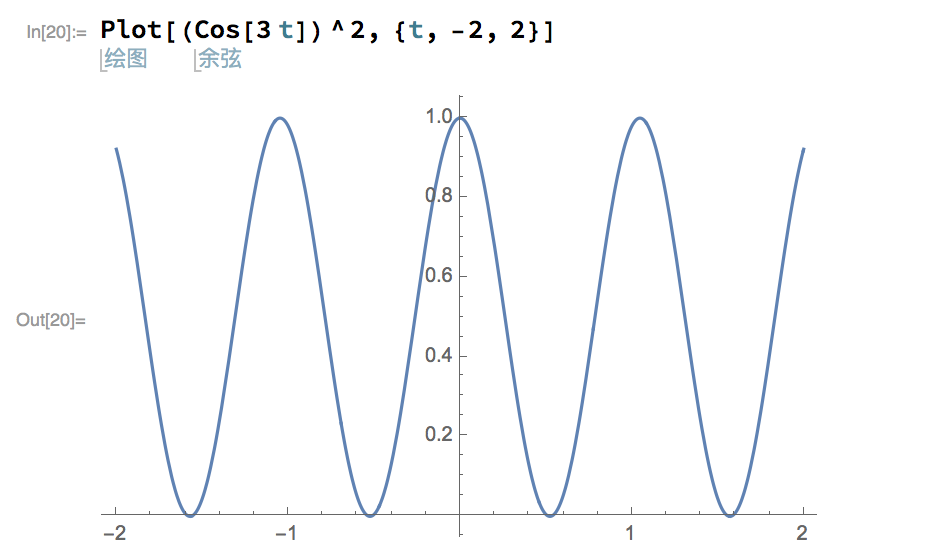
\includegraphics[width=8cm]{./Figures/20180305-cos3tsq.png}
  \label{fig:fourier-series-f-cos3tsq}
%
%  \small{Source: PBOC.}
\end{figure}

基准频率$\omega_{0} = \frac{2 \pi}{T} = 6$。已知
\begin{equation}
  \label{eq:fourier-series-expo-coef}
\begin{split}
  & \cos \left( 3t \right) = \frac{1}{2} \left[
  \exp \left( 3 i t \right) + \exp \left( - 3 i t \right)
  \right], \\
  & \hookrightarrow
  f(t) = \cos^{2} (3t) = \frac{1}{4} \left[
  \exp \left( 6 i t \right) + 2 + \exp \left( - 6 i t \right)
  \right], \\
  & \hookrightarrow
  \tilde{f}_{\nu} = \frac{1}{4 T} \int_{0}^{T}
  \exp \left( -i \nu \omega_{0} t \right)
  \left[
  \exp \left( i \omega_{0} t \right) + 2
  + \exp \left( - i \omega_{0} t \right)
  \right] \, \mathrm{d} t.
\end{split}
\end{equation}

结合Appendix\todo{做一个reference}中正交性关系的介绍可得,上式变为
\begin{equation*}
  \tilde{f}_{\nu} = \frac{1}{4}
  \left[
  \delta_{\nu,1} + 2 \delta_{\nu,0} + \delta_{\nu,-1}
  \right],
\end{equation*}
换句话说,傅里叶级数的系数$\tilde{f}_{\nu}$只有在$\nu = \left\{ -1, 0 ,1 \right\}$时不等于$0$。那么,将$f(t)$用傅里叶综合形式\todo{做一个ref}写为
\begin{equation}
  \label{eq:fourier-series-expo-coef-cal}
  \begin{split}
    f(t) & = \sum_{\nu} \tilde{f}_{\nu} \exp \left( - i \nu \omega_{0} t \right) = \frac{1}{4} \exp \left(i \omega_{0} t \right) + \frac{1}{2} + \frac{1}{4} \exp \left( - i \omega_{0} t \right) \\
    & = \frac{1}{2} \left[ 1 + \cos \left( \omega_{0} t \right) \right] = \frac{1}{2} \left[ 1 + \cos \left( 6 t \right) \right],
  \end{split}
\end{equation}

结合三角函数关系,上式还可以做进一步简化
\begin{equation*}
  \cos^{2} \left(3 t \right) = \frac{\cos \left( 6 t \right) + 1}{2}.
\end{equation*}

\subsubsection{傅里叶余弦级数}
\label{sec:fourier-series-sin-coef}

\eqref{eq:fourier-series-expo-coef-cal}将$f(t) = \cos^{2} \left( 3t \right)$分解为一个余弦项和一个常数项之和,没有正弦项。事实上若方程$f(t)$是偶函数,傅里叶变换后常常是没有正弦项的。反之亦然。我们将两种情况分别称为傅里叶余弦级数(Fourier cosine series)\index{Fourier cosine series \dotfill 傅里叶余弦级数}和傅里叶正弦级数(Fourier sine series)\index{Fourier sine series \dotfill 傅里叶正弦级数}。

有时候原始方程本身既不是奇函数也不是偶函数,但有可能通过坐标点的移动来变成奇或偶函数。如$T$-周期方程
\begin{equation*}
  f(t) = \begin{cases}
  0, & 0 < t < \frac{T}{2}\\
  1, & \frac{T}{2} < t < T
  \end{cases}
\end{equation*}
非奇非偶。可以设一个新函数$g(t) \equiv f \left( t + \frac{\pi}{4} \right)$,使得$g(t)$变成偶函数。

更一般地说,所有方程都可以分解为奇函数、偶函数组合的形式,如
\begin{equation*}
  \begin{split}
    f(t) & = f_{\text{偶}}(t) + f_{\text{奇}}(t), \\
    f_{\text{偶}}(t) & \equiv \frac{1}{2} \left[ f(t) + f(-t) \right], \\
    f_{\text{奇}}(t) & \equiv \frac{1}{2} \left[ f(t) - f(-t) \right].
  \end{split}
\end{equation*}

举例来说如锯齿波(sawtooth wave),$T$-周期方程$f(t)$在每一个周期内都满足$f(t) = t, \quad 0 < t < T$,也即,$f(t)$的单位与$t$的单位相同,都是时间,见图\ref{fig:fourier-series-sawwave}。
\begin{figure}[htbp]
   \caption{锯齿波}
  \centering
  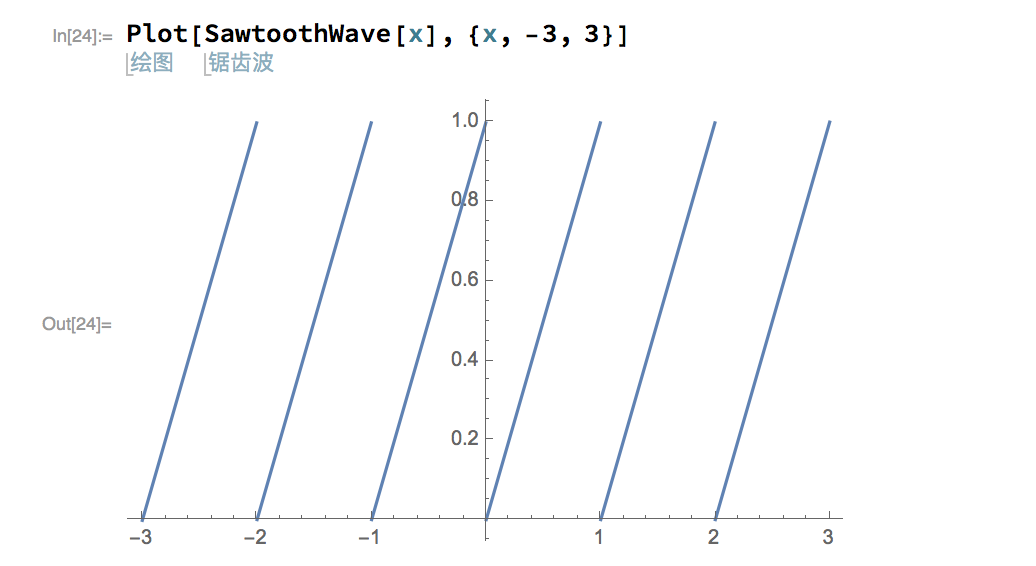
\includegraphics[width=8cm]{./Figures/20180305-sawtooth-wave.png}
  \label{fig:fourier-series-sawwave}
%
%  \small{Source: PBOC.}
\end{figure}

该方程的傅里叶级数
\begin{equation*}
  \begin{split}
    f(t) & = \sum_{\nu = - \infty}^{\infty} \tilde{f}_{\nu} \cdot \exp \left( i \nu \omega_{0} t \right), \quad \omega_{0} = \frac{2 \pi}{T}, \\
    \hookrightarrow \tilde{f}_{\nu} & = \frac{1}{T} \int_{0}^{T} f(t) \exp \left( - i \nu \omega_{0} t \right) \, \mathrm{d} t = \frac{1}{T} \int_{0}^{T} t \exp \left( - i \nu \omega_{0} t  \right) \, \mathrm{d} t.
  \end{split}
\end{equation*}

上式中$\tilde{f}_{\nu}$的值随着$\nu$的取值而不同,具体说来:
\begin{equation*}
  \tilde{f}_{0} = \frac{T}{2}, \quad \nu = 0,
\end{equation*}
\begin{equation*}
  \begin{split}
    \tilde{f}_{\nu} & = \frac{1}{T}
    \left[
    - \frac{1}{ i \nu \omega_{0}}
    \left| t \exp \left( - i \nu \omega_{0} t \right) \right|_{0}^{T}
    + \frac{1}{ i \nu \omega_{0}}
    \int_{0}^{T} \exp \left( - i \nu \omega_{0} t \right) \, \mathrm{d} t
    \right]  = - \frac{1}{i \nu \omega_{0}}, \quad \nu \neq 0.
  \end{split}
\end{equation*}

代回可得
\begin{equation*}
    \underbrace{
    \tilde{f}_{\nu}
    }_{\text{(时间)}} =
    \underbrace{
    \frac{T}{2}
    }_{\text{时间}}
     - \underbrace{
     \frac{1}{i \omega_{0}} \sum_{\nu = - \infty}^{\infty} \frac{1}{\nu} \exp \left( i \omega_{0} t \right)
     }_{\text{单位:(1/角频率)=时间}},
\end{equation*}
不难看出,在角频率$\omega$的值较大时,$\tilde{f}_{\nu}$以等比于$\frac{1}{\left| \omega \right|}$的速度衰减。这是由$f(t)$方程的非连续性所决定的(佩利——维纳诸定理, Theorem \ref{theorem:paley-wiener-theorems})。

上式也可改为正弦余弦形式
\begin{equation}
  \label{eq:fourier-series-sin-coef-sincos}
  f(t) = \frac{T}{2} - \underbrace{
  \frac{T}{\pi} \sum_{\nu = 1}^{\infty} \frac{1}{\nu}
  \sin \left(
  \frac{2 \nu \pi t}{T}
  \right)
  }_{\eqqcolon \mathcal{A}},
\end{equation}
其中$\mathcal{A}$符合傅里叶级数的特征。若设$g(t) = f(t) - \frac{T}{2}$,则$g(t)$就是个傅里叶正弦级数了——只要$g(t)$是一个奇函数的话——将图\ref{fig:fourier-series-sawwave}垂直下移$\frac{\pi}{2}$个单位不难看出,$g(t)$也是个奇函数。

\subsubsection{吉布斯现象}
\label{sec:fourier-series-gibbs-phenomenon}
前文可见,通过加总一系列弦波方程(假定其中每一个弦波都是平滑的),可以生成图\ref{fig:fourier-series-sawwave}一般参差状不连续的锯齿方程,


\end{subappendices}
